\chapter{Approach}

\label{Chapter3}

\lhead{Chapter 3. \emph{Approach}}

\section{System overview} % (fold)
\label{approach:sec:system_overview}

The proposed system is constructed around the data flowing through it.

The system takes the data stepwise through an ingestion pipeline, importing, filtering and cleaning it, before churning it into user models. This particular part of the system is elaborated on further in section~\ref{approach:sec:data_ingestion_and_preprocessing}.

Once user models are in place, the system generates user segments. These are stored in a database for future use. There are several viable approaches to the segmentation task. These are discussed in more detail in section~\ref{approach:sec:clustering}.

As it turns out, when designing completely autonomous adaptative systems, we need more data than user segments to effectively drive the adaptive component. When considering whether to enable a feature or an interface switch, we need to know whether doing so will be advantageous to the user segment in question. This is discussed in section~\ref{approach:sec:adaptation_component}.

% section system_overview (end)

\section{Data ingestion and preprocessing} % (fold)
\label{approach:sec:data_ingestion_and_preprocessing}

Before the interesting parts of the system can start doing their work, the data needs to be transformed from \emph{a series of chronological raw events} to \emph{a set of user models}.

The amount of data can be arbitrarily sizable, and will grow linearly with user activity. The system architecture has been designed to be able to cope with this; its functional and data-driven nature should be easily adaptable to hugely scalable programming paradigms like MapReduce.

\begin{figure}[h]
  \centering
    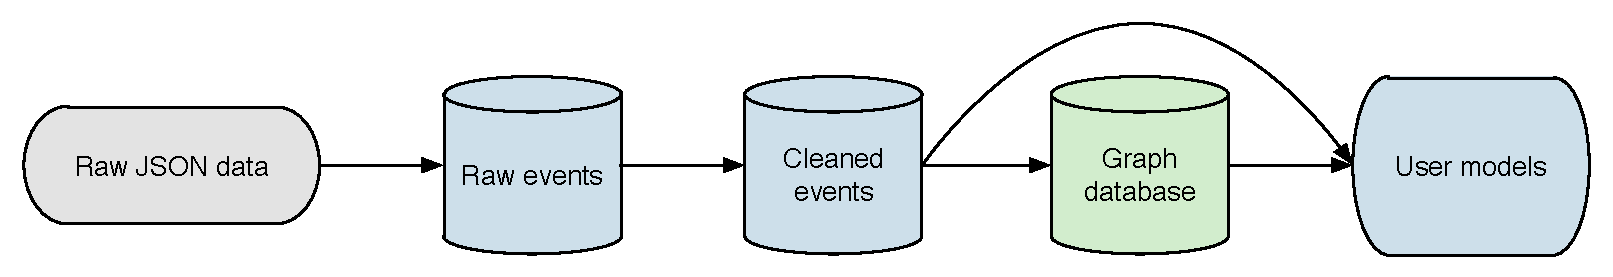
\includegraphics[width=\textwidth]{Figures/ingestion-pipeline}
  \caption{The ingestion pipeline broken into 4 steps. The color of each node indicates means of storage: \emph{Blue} indicates a RDBMS, \emph{green} indicates a graph database, whereas \emph{gray} is used to indicate flat file storage.}
  \label{fig:ingestion-pipeline}
\end{figure}

\subsection{Generating the raw data}
\label{approach:sub:generating_data}

The system input is a chronological series of raw events sent from the production system.

These are instrumented via an external analysis service called KISSmetrics\footnote{\url{https://www.kissmetrics.com/}}. It is a user analysis system designed around tracking individual users' behavior. It works by calling their REST API with the following data:

\begin{enumerate}
  \item person identifier
  \item event name
  \item user properties
\end{enumerate}

The consistency of the personal identifier has already been discussed extensively in the introductory chapters, especially section~\ref{intro:sub:anonymity_privacy}, but a short technical introduction to the actual production system is in order.

\subsection{Event instrumentation in KISSmetrics}
\label{approach:sec:event_instrumentation}

To enable effective utilization of the KISSmetrics instrumentation functionality, they supply a client library for the purpose. This client library handles a few central things for us:

\begin{enumerate}
  \item Person identity storage and loading over subsequent page loads.
  \item The low-level instrumentation of events.
  \item Simple A/B testing facilities.
\end{enumerate}

When the KISSmetrics client library is loaded, the person identity is automatically either retrieved from the browser cookies, or generated.

The identity of a person is a unique randomly generated string, which serves no other purpose than to track the identity of the browser over time. No personal data is stored, nor is it available to us.

Whenever something ``interesting'' happens, an event is sent to the KISSmetrics instrumentation service. An ``interesting'' event is anything that tells us about how the users use the service, both in terms of general activity and in terms of feature adoption. Every event is tagged with the person identity, as well as an event name and a timestamp.

The KISSmetrics service provides several analytical tools to dig into this data, thereamongst funnel reports and cohort reports -- as depicted in figure~\ref{fig:funnel-report} and figure~\ref{fig:cohort-report}.

\begin{figure}[h]
  \centering
    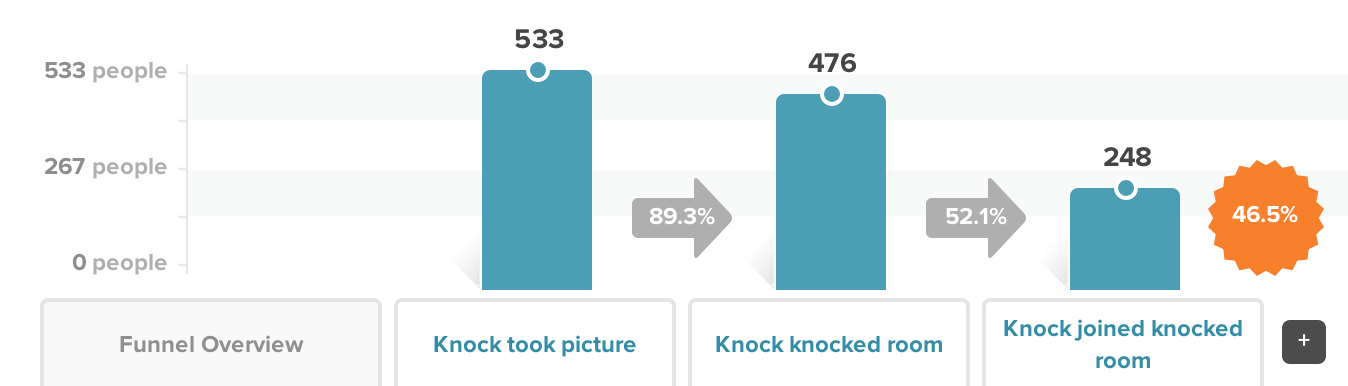
\includegraphics[width=\textwidth]{Figures/screenshots/km/funnel-example}
    \caption{Example of a simple funnel report.}
    \label{fig:funnel-report}
\end{figure}

\begin{figure}[h]
  \centering
    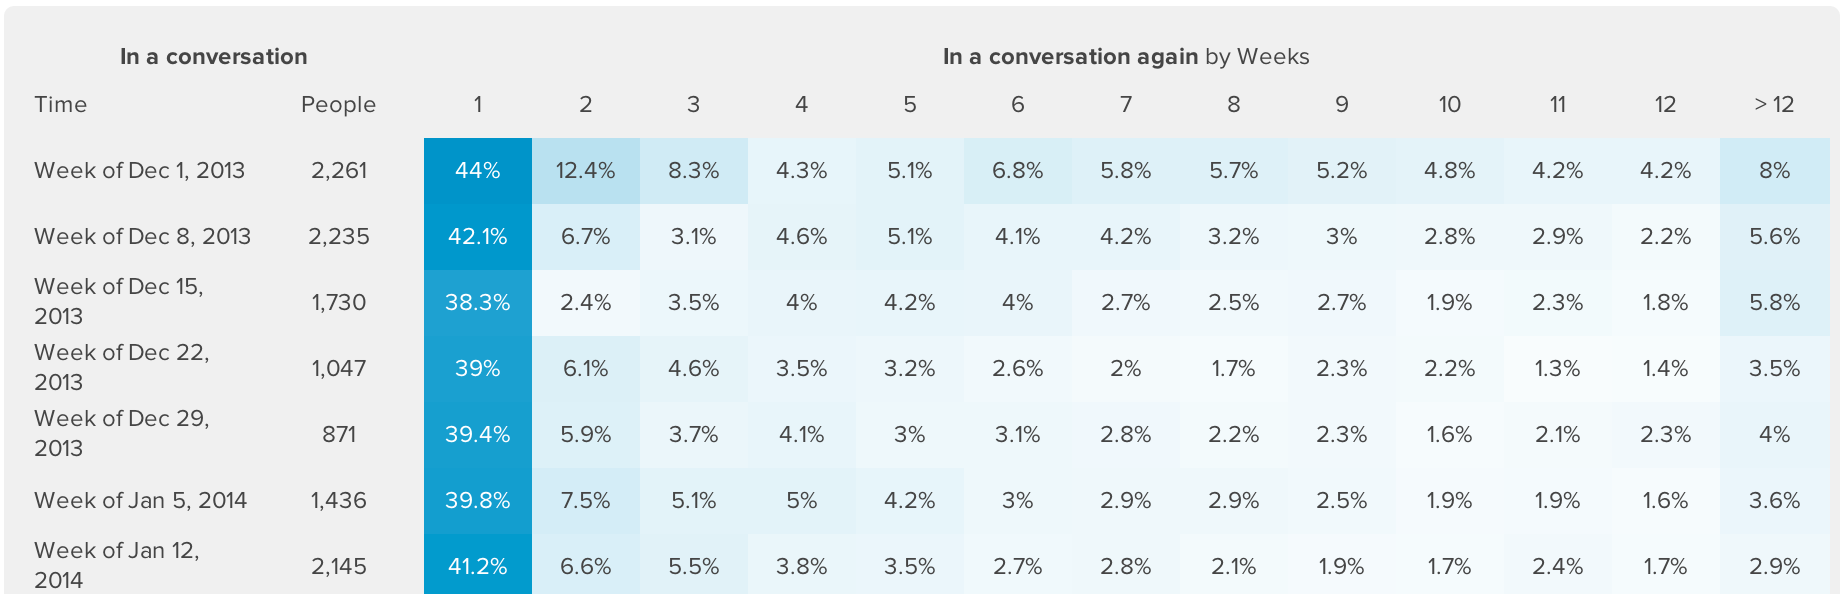
\includegraphics[width=\textwidth]{Figures/screenshots/km/cohort-example}
    \caption{Example of a cohort report.}
    \label{fig:cohort-report}
\end{figure}

\subsection{Cleaning the data}
\label{approach:sec:cleaning_data}

KISSmetrics has the ability to export raw event data to data files. This can be used to power completely customized analyses, as will be needed for our particular task.

After the raw data has been aquired, it will need to be cleaned. This is a simple process of churning through each line of each unprocessed data file, parsing and splitting its contents into appropriate data fields, and inserting it into a database.

To facilitate the compilation of network-related user model features, conversation data was loaded into a graph database to enable querying of network structures. In the RDBMS handling the other data, this presented itself as a computationally unfeasable task.

% section data_ingestion_and_preprocessing (end)

\section{User modeling} % (fold)
\label{approach:sec:user_modeling}

To find clusters of users, we first and foremost need to quantify them. More specifically, we want to represent each user as a feature vector in an $n$-dimensional space.

\subsection{Feature selection}
\label{approach:sec:feature_selection}

Given the types of events being collected, we landed on compiling the following features:

\begin{enumerate}
  \item First degree conversation partners
  \item Second degree conversation partners
  \item Inviter
  \item Invitee
  \item Conversations
  \item Rooms used
  \item Rooms claimed
  \item Roomnames generated
  \item Chat message sent
\end{enumerate}

To generate user models, the stream of event data needs to be mapped to its associated users for aggregation. This is a classic MapReduce task~\cite{Dean2008} easily solved using simple functional techniques, and did not present itself as a particularly interesting problem, albeit a computationally heavy one.

To summarize, the transformation in this step started with data in the form of \eqref{pre_user_model}.

\begin{equation}
  \langle \text{event}, \text{timestamp}, \text{person}, \text{metadata} \rangle
  \label{pre_user_model}
\end{equation}

And ended with data in the form of~\eqref{post_user_model}.

\begin{equation}
  \langle \text{person}, \text{feature}, \text{value} \rangle
  \label{post_user_model}
\end{equation}

\section{Clustering the users}
\label{approach:sec:clustering}

We assume the following hypothesis holds, as a basis for the clustering approach to the user adaptation problem:

\begin{hypothesis}
The more similarly two people use a service, the more likely they are to respond similarly to it changing.
\end{hypothesis}

Thus, we want to segment the users in the following way: users in each segment should be as similar as possible, and as dissimilar those in other segments as possible. This scheme fits well with the two criterias for selecting an optimal clustering scheme, as described by Berry and Linoff~\cite{Berry1997}.

@TODO: Remember the bias introduced in section~\ref{survey:sub:generality}.

\subsection{Choice of algorithms}
\label{approach:sec:clustering_algorithms}

Three algorithms were implemented and experimented with: DBSCAN, mean-shift, and k-means. Of these, the k-means clearly proved itself as the most effective one, and as it also managed to produce adequate and meaningful results, it was chosen as the principal algorithm.

\subsubsection{The k-means clustering algorithm}
\label{subs:kmeans}

The k-means clustering algorithm is arguably one of the most intuitive clustering algorithms.

It takes as input a preset number of clusters, $k$, a similarity measure function, and a set of data vectors. Initially, it randomly chooses $k$ data vectors as centroids as a starting point for the process, before repeatedly performing a two-pass operation adjusting the centroids until convergence.

Figure~\ref{fig:k-means} shows a simple python-esque implementation of the algorithm.

\begin{figure}[h]
  \begin{minted}[gobble=4]{python}
    def kmeans(K, distance_fn, vectors):
        N = len(vectors)
        cluster_members = {}
        memberships = {}

        # Initially set centroids to random data vectors
        centroids = [vectors[randint(N)] for _ in xrange(K)]

        while True:

            # Assign each data vector to the closest cluster centroid
            for vector in vectors:
                k = argmin(K, lambda k: distance_fn(centroid[k], vector))
                if not memberships[vector] == k:
                    cluster_members[memberships[vector]].remove(vector)
                    cluster_members[k].append(vector)
                    memberships[vector] = k

            # Set each centroid to the mean of its members
            previous_centroids = centroids
            for k in xrange(K):
                centroids[k] = mean_vector(cluster_members[k])

            # Stop computing if we've achieved convergence
            change = 0.0
            for k in xrange(K):
                change += distance_fn(previous_centroids[k], centroids[k])
            if change < CONVERGENCE_THRESHOLD:
                break
  \end{minted}

  \caption{The k-means algorithm}
  \label{fig:k-means}
\end{figure}

\subsection{Evaluating cluster quality}
\label{approach:sub:evaluating_clusters}

@TODO: Davies-Bouldin index etc.

\subsection{Normalizing axes}
\label{approach:sub:normalizing_axes}

\subsection{Storing clustering results}
\label{approach:sub:storing_results}

\section{Identifying adaptable product features}
\label{approach:sec:identifying_adaptability}

Ideally at this point, we have identified several significant clusters of users. Now we want to adapt the product to better suit each user, based on the cluster he or she belongs to.

Given a set of candidate product alterations $A$, we want to give each user the combination of these that maximizes some performance measure $P$. However, we arguably have no predictive bias to start us off on solving this.

The approach taken in this implementation is a simple one, which relies on conducting a single A/B test up front for each candidate product alteration. The important part during this phase is to log each selected alteration variant along with the same person identifier used for other event instrumentation, as discussed in section~\ref{approach:sub:generating_data}.

This approach enables us to see up-front whether there are any significant variances in feature adoption between the clusters. If there are, we can adapt the service by selecting the more successful variation of the feature for all users in the relevant clusters. If not, we have a feature that affects all users equally -- at least with regard to cluster granularity.

\subsection{Evaluation metrics} % (fold)
\label{approach:sec:evaluation_metrics}

When considering which variation of a product feature to prefer, we need to be able to measure their relative success rates.

As for any user-facing product, the main objective is achieving user happiness. However, user happiness is hard to objectively define. For a service like appear.in, though, activity level should serve as a pretty clear indicator of user happiness -- unhappy users have more than enough alternative applications that cater to their needs.

Simply put, we basically assume that the following hypothesis holds:

\begin{hypothesis}
  Happy users use the service more than unhappy users.
\end{hypothesis}

Furthermore, we seldom need a measure of \emph{user happiness} to determine the relative success of variations of a product feature. Some parts of the product have clearly defined goals themselves.

The perhaps most obvious example of this is the landing page, whose main objective is to get people to try out the product. We can define the performance of the landing page in terms of the percentage of users that continue on to try out the product.

\section{Adaptation component} % (fold)
\label{approach:sec:adaptation_component}


\subsection{Applying the personalized feature set} % (fold)
\label{approach:sec:applying_the_personalized_feature_set}

Description of the FlagService model.

% section applying_the_personalized_feature_set (end)

\subsection{Visualizing effects} % (fold)
\label{approach:sec:visualizing_effects}

% section visualizing_effects (end)

% section adaptation_component (end)

\subsection{Differentiating product features} % (fold)
\label{approach:sec:differentiating_product_features}

% section differentiating_product_features (end)

\section{Evolving the user models} % (fold)
\label{approach:sec:evolving_the_user_models}

\subsection{Multi-arm bandits}

\subsection{Tracking individual treatment}

% section evolving_the_user_models (end)

\section{Visualization requirements (?)} % (fold)
\label{approach:sec:visualization_requirements}

% section visualization_requirements (end)
